%%%%%%%%%%%%%%%%%%%%%%%%%%%%%%%%%%%%%%%%%%%%%%%%%%%%%%%%%%%%%%%%%%%%%%%%%%%%%%%%
% This chapter covers the design aspects, include design for data processing
% and the visual design
%
% - Can probably expand interaction section, particulary spatial-interaction
% - Should consider rewording 'stage 2: tagging'
% - Should probably talk about active versus inactive versus context objects 
%   in the 3D visualization section
% - Should probably talk about rational for picking 3D space first before
%   going into too much detail
%%%%%%%%%%%%%%%%%%%%%%%%%%%%%%%%%%%%%%%%%%%%%%%%%%%%%%%%%%%%%%%%%%%%%%%%%%%%%%%%
\chapter{Design}
This chapter covers our visual design process and our rationals for our
decisions. The first section describes our treatment of the dataset and how we
calculate our scoring functions. The second and third covers the visualization
interface in detail, describing our visual encoding and how each interactive
widget's design tie back to our requirement as listed in the previous chapter.
Lastly, we describe our design for higher level functions that can be used to
detect trends and to make comparisons across different entities.


%%%%%%%%%%%%%%%%%%%%%%%%%%%%%%%%%%%%%%%%%%%%%%%%%%%%%%%%%%%%%%%%%%%%%%%%%%%%%%%%
\section{Data Processing}
In order to create our visualization, first we must be able to process and
extract semantics from our text collection. Our processing is broken down into 
three different stages, normalization, preprocessing and an
extraction/scoring stage. The normalization stage removes irrelevant entries and
attempts to clean up the text as much as possible. The preprocessing stage deals
with normalizing the text and building a vocabulary of keywords that are used to
represent the entities found in the document. The extraction/scoring stage
scores each document the number of occurring keywords. Lastly, the final stage
involves segmentation of \threed models into subgroups such that each group can
be semantically mapped against the keywords.
 

%\subsection{Stage 0: Normalization}
%From a preliminary analysis of the dataset, we found entries that are
%irrelevant with respect to our subject data. There entries can be identified by
%a type field and filtered out before any type of processing takes place. On top
%of that, the text descriptions are quite difficult to read, because they are
%capitalized and have have trailing suffix characters that are not English nor
%are they domain specific terms. We use regular expressions to perform upper
%and lower case conversions such that the descriptions would be atypical of
%English text. To remove the suffix characters, we created a dictionary of stop
%words.


\subsection{Stage 1: Bootstrapping}
Before any logical processing can take place, we spent some time doing
preliminary analysis, looking at the data text, their format and how they have
evolved over the life span of the data repository. We performed several
normalization tasks: One, we used regular expressions to convert the text, which
is call caps, to regular case format. Secondly, we remove suffix characters that
appear at the end of the text paragraph, that, as far as we know contributes
nothing to the incident context. Although we changed the underlying text, the
normalization process improves readability, and allows us receive meaningful
output from natural language parsers.

The first issue was to devise a method for extracting physical entities; a
document can contain multiple entities, but not all of which are related to the 
subject matter. On top of that, many entities can have implicit hierarchical 
relations, such as relation between component and its subcomponents. This 
relation is important because it enables logical groupings which are useful for
high level overviews.

Our entity extraction process leverages the WordNet database, a lexical English
database that stores nouns, verbs, adjectives and their relations among each
other \cite{WORDNET}. In order to get a comprehensive list of physical entities, we use the meronym 
relation in WordNet. A meronym describes a ``part-of'' relationship between two 
nouns, for example, a brake is a part of a wheel, and a wheel is a part of the 
automotive vehicle. All together, the meroynomy relationship forms a hierarchical 
structure where the most general part forms the root node, while the most specific 
parts form the leaf nodes. We use two common words pertaining to cars to bootstrap 
the hierarchy : ``car'' and ``vehicle''. From this we extracted two tree
structures rooted at ``car'' and ``vehicle'' respectively, we then merge the two
hierarchies, assuming that ``car'' and ``vehicle'' are equivalent. 

While this process extracts a fair amount of physical entities, an analysis of
sample dataset showed that it is not representative of the entities being
mentioned in the documents. The primary reason for this is due to the use of synonyms in the documents, 
where the entity words in question are using an alternative names. To alleviate
some of these confusion, we additionally extract the synset relations from WordNet. A
synset is a set relationship that describes words that are semantically
equivalent of one another, for example ``limo'' and ``limousine'' both describe
the same type of object and thus belongs to the same synset group. For each word
in our current collection, we replace it with its respective synset.

The addition of synsets into the vocabulary gave us a comprehensive number of
keywords, however it also created undesirable noises. Manual examination of data
sample reveals that there are still disconnects between the dictionary
vocabulary and real world vocabulary. The next section we will describe how we
overcome these issues.

    % ===== Figure =====
	\begin{figure}
	   \centering  
	   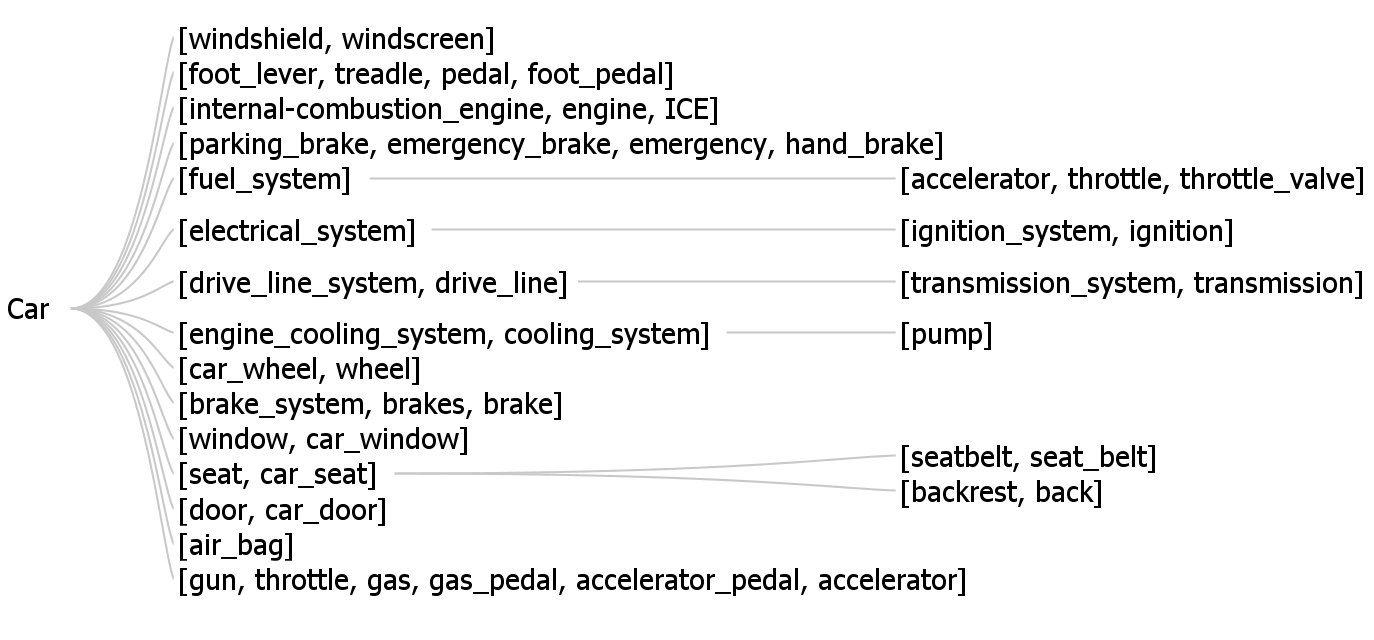
\includegraphics[width=\columnwidth]{meronomy.png}
	   \caption{An example of the meronomy plus synset structure}
	   \label{figure:meronomy}
	\end{figure}
	% ==================

\subsection{Stage 1: Manual Processing}
As an additional step to augment our keyword vocabulary, we perform two manual
steps:
\begin{itemize} [noitemsep]
  \item Removal of nouns that are too generic from the vocabulary.
  \item Preprocess the documents and mine for any missing nouns.
\end{itemize}
The first step deals with the removal of keywords that are not considered to be
physical objects under typical usage, for example WordNet hierarchy of a
vehicle contains ``first'', ``second'', ``third'' and ``fourth'', which
describes the first, second, third and fourth gears respectively. Including
these words will likely result in over-counting the number of occurrences of
gears because they are used in every day speech. We also removed several
acronyms that will likely cause ambiguities, for example ``ice'', which is short for internal-combustion-engine,
will cause issues if the document is about ice, the solid state of water. They
are therefore removed from the keyword dictionary. 

The second step deals with any possible missing keywords that are not in WordNet
meronyms. We attempted to detect these semi-automatically with natural language 
processing techniques. We first perform part-of-speech (POS) tagging on our document 
corpus. POS taggers look at the grammatical structures of text and break down 
sentences into lexical categories such as nouns, verbs and adjectives. We use the 
POS output and tie them back to the original text, extracting the nouns and 
compound-nouns. We perform this step for all the documents in the corpus and 
count the number of occurrences for the nouns and compound-nouns. We then manually 
exam the top occurring nouns and add them into the hierarchy where we believe 
would be appropriate.

\subsection{Stage 1: Limitations}
While we believe this extract process is a plausible method for building the
vocabulary, we acknowledge that WordNet is not the definitive authority for our 
problem domain, nor would it be for any specific domain. The automatic
extraction can be used as a starting point. The keywords vocabulary should be
extended and further refined by consulting experts that works in the problem field. 

\subsection{Stage 2: Tagging}
For the actual matching, we use an open source, off the shelf snowball
stemmer\footnote{http://snowball.tartarus.org/} before any matching takes
place. Stemming is a process of reducing the words to their root forms. Finding the root is important because it unifies the singular 
and plural forms, as well, it converges various forms without the need to add 
additional vocabulary to our keywords. For the purpose of string matching, we 
perform stemming on both documents and key word vocabularies.

For the document text, stemming is performed on all string tokens and not
limited to nouns. This has both positive and negative effects. In our data, 
there are many word tokens with both noun and verb forms, for example ``braking
malfunction'' can be correctly associated with the keyword ``brake'' with
stemming. On the other hand this also introduced false positives, the word
``lock'', which refers to the component, is falsely picked up when the text describe components
``locking up''.

We have also looked at tagging explicit casual relations. Using the dependency
parser extension, the output is a tree-like structure that can be used to infer
word dependencies. In practice this did not work very well; informal languages,
spelling mistakes and grammatical errors result in incorrect dependency parse
trees. We ultimately opted to go for a more general approach, where we tag each
physical entities as well as co-occurring entities within the same document.


\subsection{Stage 2: Scoring Scheme}
Once we have identified the entities in each document, we can compute each
entity�s importance score. We denote the importance score of a physical entity 
as the number of times it is mentioned within the document corpus. We have two 
variations of importance score: occurrence  and co-occurrence. Within our
problem context, the occurrence scores denotes the components that are most prone to failure, while 
the co-occurrence suggest causal relationships among the objects.

Let G be a (possibly empty) set of objects that are in the keyword hierarchy and
c be a single object in the hierarchy. We define a scoring function S(c, G) to be 
the total number of documents that have at least a single mention of c and G. Thus 
when G is the empty set the score is the absolute occurrence score (every document 
contains an empty set). When G is non-empty the score reflects the co-occurrence 
strength among a set of components. For clarity we illustrate this with a few examples:
\begin{itemize} [noitemsep]
  \item $S(engine, \{\})$: The absolute strength of ``engine'' component in all
  documents
  \item $S(engine, \{engine\}$): The strength of ``engine'' relative to
  ``engine'', thus the same as the above
  \item $S(engine, \{brake\})$: The number of times engine keyword is mentioned
  when brake keyword is mentioned as well. Thus, mathematically,  $S(brake,
  \{\}) \geq S(engine, \{brake\})$
\end{itemize}

Each document is only counted once per physical entity, this was done to
discourage biases coming from longer documents where the entities are
repetitively mentioned.


\subsection{Stage 2: Limitations}
For this prototype, we gave the same score weighting to each objects. This is a 
subjective measure because not all parts are created equal. For example: if window 
is mentioned 10 times and the engine mentioned a single time, does that mean we 
should pay more attention to the window component? An extension to this work
would be to devise an appropriate weighting scheme for our problem domain.

Another limitation is the vocabulary set itself, while we are only storing nouns 
as keywords, it would be interesting to look at verbs as well. For example, 
``stalled'', ``stalling'' are typically associated with engine object. Adding
verbs into our dictionary would give more flexibility and accurate results.

\subsection{Stage 3: Model Segmentation}
We use geometric models that compose of triangular mesh groups, where each mesh 
group can be uniquely identified and semantically mapped to our keyword ontology. 
The segmentation is done manually, with consultation of car schematics when it 
was not clear where the parts located. Where the model is missing parts, 
we add placeholder geometries.

We have chosen to use a sedan model as the starting point of our visualization. 
This was chosen based on the fact that sedans are the most common class of 
vehicles and best represent our data. We acknowledge that different types of 
vehicles may have different spatial arrangement of their components, we hope to 
remedy this as more vehicle models are processed.


%%%%%%%%%%%%%%%%%%%%%%%%%%%%%%%%%%%%%%%%%%%%%%%%%%%%%%%%%%%%%%%%%%%%%%%%%%%%%%%%
\section{Visual Design}
The following sections discuss our user interface and design decisions. In
summary, our interface is composed of five major components as seen in
\ref{figure:overview}

\begin{itemize} [noitemsep]
  \item Stylized Visualization: The central point of the visualization system is
  a stylized rendering representing the physical entities in the text documents,
  the visualization can be zoomed and rotated to explore different viewing
  perspectives. Each entity is rendered with respect to a function which denotes
  its importance, we explore different rendering styles to take advantage of
  viewers' preattentive perception, allowing them to quickly uncover the
  important subject matters.
  
  \item Time Filter: The filter is composed of two independent range sliders
  with different granularity: year and month. The filter allows viewers to
  adjust the time range for the visualization. Accompanying each range slider is
  a histogram showing the accumulated volume of complains over a time period.
  The widget itself is place at the top-left of the display space.
  
  \item Hierarchy Filter: The hierarchy filters are placed at the
  bottom portion of the display akin to a series of drop-down menus. These are 
  designed specifically for our data of automotive complaints. The
  hierarchy filters allow successive query refinement by organizational
  hierarchies of manufacturers, going in the order of : Vehicle Manufacturer,
  Vehicle Make, Vehicle Model and Vehicle Year. Hierarchy filter is also used to
  select two different vehicle types in comparison mode.

  \item Lens Widget: The lens widget is used for exploration and
  visually querying the visualization. When the lens is hovered over the
  \threed visualization, additional information of the objects underneath the
  lens are displayed as heatmap charts placed around the lens circumference.

  \item Heatmap Widget: The heatmap widget displays time-series data, it
  is similar in function to the histogram of the Time Filter widget, but
  at a component level. Volume for each period is encoded as a shaded square and
  arranged into a grid pattern to match the selected time range. The heatmap
  offers the viewer several different perspectives to see trends and find outliers in the data.
  
  \item Document Widget: The document widget displays the source text documents.
  The panel displays documents relating to the current selected objects and 
  highlights all component keywords.
\end{itemize}

\begin{figure}
 \centering  
 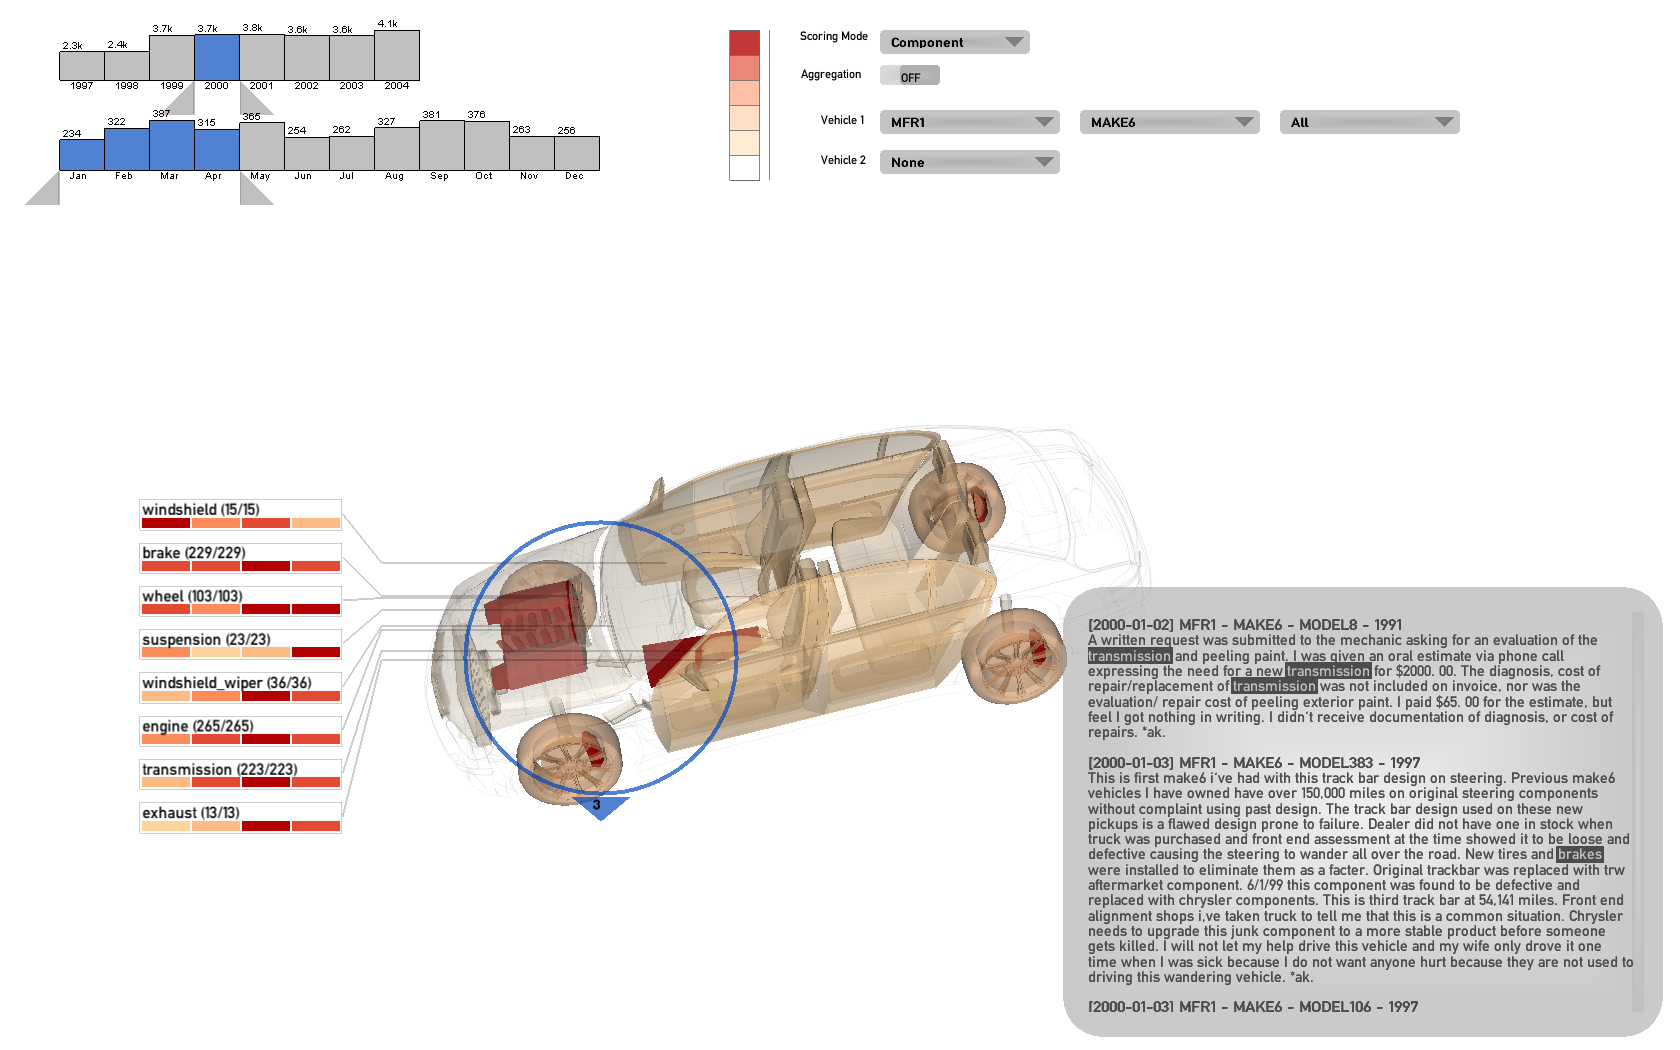
\includegraphics[width=\columnwidth]{overview.png}
 \caption{System Overview}
 \label{figure:overview}
\end{figure}

In the following subsections we will describe each visualization components in
more detail, the trade offs and choices we made and our justifications.


\subsection{Design Rational}
A major part of our design for this thesis is the mapping of abstract semantics
onto realistic looking, \threed models. But this can also be a source of
complication, we have to deal with the additional difficulties of navigating in
three dimensional space,  as well as work around perceptual limitations. So why
use \threed models in the first place? We hypothesize that the additional sense of
realism helps people see and communicate better then when they are working with
raw text or data in abstract forms. The familiarity with how the physical
entities look means people do not have to learn additional visual mappings. Communication may
be eased because there is a shared common ground among the different parties.
Proximal relationships are also easily perceived if they have realistic spatial
mappings and can encourage more thorough exploration of the dataset. These
advantages are not readily present in abstract representations, while with
careful design it is possible to overcome the pitfalls of perceiving \threed graphics.

Yet another argument is that the use of a set of \twod images can also convey
realism, our opinion is that they lack the expressive power and playfulness of a
fully rendered \threed model. Flat image representation would likely result in
multiple images, to cover different sections of the entities and viewing angles,
this can result in more cognitive load due to the viewers switching between
images to get an overview.


\subsection{Visual Mapping}
Because our visualization environment makes use of 3 dimensional space,
extra care are taken into account for the selection of visual variables. Not all 
variables are appropriate, shape, position and orientation are inherently used 
to represent the geometries on the virtual model, a double encoding of these
variables is likely going to lead to confusion, compromising the ability to
interpret the visualization, or destroy any resemblance of the virtual model to
its real world counterpart. Thus these are rejected in the early part of our
design. Size is an interesting one, in theory size can support most of the
characteristics. However it is implied that all the objects of the same value have the equal size, 
which is certainly not the case for physical objects with sub components. Colour 
and value variables are not used to represent the virtual model, in the sense that 
they are not a part of the  basic geometry building blocks of vertices, line-segments 
and polygons. We found colour and value to be appropriate for our visualization, 
while they do not provide a sense of quantitative measure, the capability to see order, 
selective and associative characteristics makes them a logical choice for an overview visualization. 

Lastly, textures present an interesting option, textures can carry additional 
characteristics, particularly descriptive attributes. It may be possible to use 
textures to simulate certain effects, for example a rusty surface. Nonetheless,
textures do not possess order or quantifiable characteristics and was not
included in our design. However it may be interesting to use textures for
visualizing individual document, we leave this idea as future work.

\subsection{Stylized Visualization}
%Data comes in many different dimensions, include those with spatial attributes
%and those with abstract attributes. Our innovation is to show these spatial 
%vocabulary as they would exist in the physical world, while using the abstract 
%attributes as rendering parameters. For tasks related to word frequencies and 
%other scores, we hypothesize that people will be able to see, and communicate 
%better than in raw text formats because they are working with a familiar form. 
%Proximity-based clusters formed in the spatial dimension would also encourage 
%exploration of these areas that may otherwise go undetected. In our visualization, 
%we use \threed models comprised of segmented sub-mesh groups that link to our
%part-of relation hierarchy of component keywords.

In order to enhance the message carrying capacity of the visualization, we
considered several NPR techniques as a medium to created a more expressive
illustrations. We associate the entity score with either a NPR technique, or use
the score as a parameter into a NPR function. In accordance with our requirement, the encoding
scheme should be clear and distinguishable by visual examination (Requirement
R1) while maintaining the real world aspects. Our effects include varying
stroke, halo/glow, colour variations, and transparency effects. 

We chose colour mappings as our primary visual encoding which denotes the
strength of non-zero scored components, and use other techniques to denote
selection and overall context.

Designing a colour scheme for the encoding of the virtual component objects
presented several design trade-offs. We colour each object by mapping its score 
to a linear diverging yellow-orange-red hue scale, which is further divided into 
six discrete scoring bins. This has both advantages and disadvantages. The
advantage is that it is much easier to distinguish a small number of hues than a
continuous hue scale. The disadvantage being that we lose the ability to compare
the relative distance between the buckets. For example, imagining the case were
we have low value in bucket 1 and high value in bucket 2, this is equivalent
to high value in bucket 1 and low value in bucket 2. We partially mitigate
the ambiguity by allowing the viewers to extract exact numerical values with the
heatmap widgets, we will discuss this further down. We display the discrete hue
scale as an on-screen legend at the bottom-left of the display screen.

We recognize that blending different hues in \threed space does not necessarily
produce a result which preserves the original hues, and can potentially lead to
distracting visual artifacts. Different hue preservation schemes
exist\cite{Chuang2009} but were not implemented for this prototype due to the
added performance complexity (Hue adjustments are done at per pixel levels).
Due to known issues with blending, we have tried to use a single hue grey scale 
with varying brightness, but we found that it was somewhat difficult to distinguish 
overlapping or contained objects. Subjectively speaking, single-hue also looks
less aesthetically pleasing, the entities did not have the ``pop-out'' effect
as we seen with multi-hue schemes. Thus we decided that using  a multi-hue
scheme was more appropriate, despite the potential blending artifacts.

A second design trade-off was whether lighting effects should be used. Lighting
effects such as specular lighting can create distractions because it can create 
highlights in places of little or no significance. Without any realistic
or simulated lighting effects, the visible colour of the components exactly
matches the colour assigned to the score (and as seen on the legend).
However, without any sort of lighting, particularly some type of diffuse lighting, 
the \threed nature of the model, and the details of various components are not
sufficiently visible. Adjacent objects that share the same score appear to be glued together 
as a single component, adding boundary outlines helps but creates undesirable
visual clutters. When lighting effects are enabled, the objects are easily
distinguishable as lighting provides a clear silhouette. However, this type of lighting modifies 
the colour based on the incidence angle of the light rays, thus it no longer matches 
the assigned colour. Ultimately our design decision is that object recognition and 
familiarity is important to us. Thus, by restricting the number of hues (6 buckets) 
and using soft white light, we contend that the lighting effects do not disturb 
the colour perception enough to obscure which hue-bin the component belongs to. 
We made the design decision that the benefits of enabling lighting to visually 
resolve the components outweighed the negative effect of shifting colours away 
from those displayed in the onscreen legend. The results of our design choices
can be seen in Figure \ref{figure:visualEncoding}.
 

    % ===== Figure =====
	\begin{figure}
	   \centering  
	   \includegraphics[width=\columnwidth]{visual_encoding.png}
	   \caption{Showing the visual design trade offs}
	   \label{figure:visualEncoding}
	\end{figure}
	% ==================


In our design, we want to make all important objects visible (See requirement
R1), these includes objects partially or fully occluded by another object, and 
objects that are contained within others. The first case can be partially solved 
by altering the viewing distance and viewing perspective on the visualization,
whereas in the second case no amount of viewing adjustment will solve the
occlusion issue. To address this problem, we double-encoded the importance score
as both the colour and transparency values. The transparency value of each
object is proportional to the object�s score, such that the higher scored
entities appear more opaque, while the lower scored entities appear more
transparent. The maximum and minimum transparency values are capped at both ends
such that no objects are completely opaque or completely transparent. Our
transparency scale is slightly weighted to give more emphasis for more
frequently occurring entities. One caveat of rendering translucent geometries in
\threed space is that ordering of geometries becomes important for blending to
work correctly, out-of-sequence geometries appear to lose their depth cues when
blended together. We will discuss this effect, and solutions in further detail
in the implementation section.


The zero score has a special semantic in our prototype. When an entity's score
is zero, this indicates that there are no known references of the entity that 
matches the query. We could choose to not render this object at all, which
would remove visual clutters. However, these zero scored objects are still
valuable because they provide background context for the non-zero entities.
Without them it may be difficult for the viewers to understand what they are
looking at. Thus, in this instance we want to denote that these entities are not
important, while at the same time minimize occlusion. Rather than using colour
and transparency as our graphical effects, we extract edge information from
their corresponding geometries and rendering them in a faint, ghostly-looking
outlines. We use just-noticeable colour in order to provide context without
distractions \cite{BAR2007a}. It is important to note that zero objects are
purely graphical artifacts and they do not partake in any user interactions.


Since we are dealing with \threed geometry, it can be tempting to apply other
types of techniques. For example we attempted to encode the importance and other 
numerical semantics into a geometrical distortion function that can be applied
directly onto a \threed mesh. In practice, this does not work well for visual evaluation:
in general, objects are of different shapes and sizes, applying a small distortion 
is not entirely obvious while a large distortion can destroy the familiarity of 
the form. Yet another problem is that it is not possible to order or quantify by 
shape \cite{BER1983a}, which makes the distortion a qualitative measure instead
of a quantitative one. In addition, the ability to read quantitative value from a 
distortion field presumes that the viewer has a mental model of what the object 
looks like without any distortions, an assumption that we cannot make with our 
intended audiences.  However distortion remains an interesting possibility because 
we may use distortion to visually paint the action words, testing this will be 
part of our future work.


\subsection{Hierarchy Filter Widget}
The hierarchy widget is designed to model inclusive relationship, in particular,
it is specifically designed to address the need to for comparison(R2) and trend
finding(R3). For our problem domain, this relationship is represented as the
organizational hierarchy. Our data contains four such fields: manufacturer,
make, model and model year. For example: Civic (Make) belongs to Honda
(Manufacturer). These filters are shown as a variant of the combo boxes which
supports single selection, each item in the filter shows the name and the number
of documents associated with this organizational level. Rather than having the
readers comparing items by reading the numbers in text format, we double-encoded
the number of document as a horizontal histogram in similar style as the scented
widget approach in \cite{Willett2007}. The histogram bars are shaded in light
grey so they are visible but not overly distracting. The histogram makes it very
clear any outlier items, and allows reader to make relative comparison among
items. We capped the number of items that can be displayed at once, as such,
scrolling is required to navigate long list of items. When an item is selected,
we change the selected item's font type to bold and change its bar to the
selected colour(blue).



% Choose to leave the list open on selection to allow simpler selection of
% outher types ???

Each level of the hierarchy is shown in individual filters. We position the
filters left-to-right across the display space, from the most general to most
specific classification. Each filter's content is 
dependent on the selection made on its parent. For example, the ``make''
selection widget will contain different makes if ``GM'' is the selected manufacturer than
it would for ``Chrysler''.  Non-top level hierarchy widgets remain hidden from view 
until it has selectable content, thus at the start, only the top level 
(manufacturer) filter widget is visible.

The hierarchical content is dependent on the currently selected time. Our
application queries the document collection and reconstructs the hierarchy. Previous 
selected items are persisted if the items are available within the new selection 
criteria. In the case where the items do not exist, the widgets, and all their 
children widgets are hidden from view and we clear the corresponding selections.

\subsection{Time Filter Widget}
The time dimension is encoded as a histogram, with the height of each bar denoting 
the volume of unique complaints for that time period. There are several granularity 
options with our document collection: daily, weekly, monthly or yearly. From a 
preliminary analysis of the incoming volume of complaint documents, we found that 
daily and weekly granularity resulted in too much noises, there are insufficient
amount of data at that level to form visually detectable trends and other
interesting patterns. Thus we selected to use month and year as our base time
periods. The widget is made up of two sliders. The top slider represents time
period in years, and the bottom slider represent time periods in months. Text
labels at the top of each bar give the numerical representation of the volume of
documents.

Time selection is not continuous, but rather in a block like manner. Multiple
years and multiple months can be selected simultaneously; when more than one
year is selected, the values on the month's histogram become the accumulated sum
of the month across the selected years. There were two motivations for this
design approach: One, this allows us to analyze a large time frame without
sacrificing too much screen real estate. Two, because the number of months is
static, viewers can compare month-to-month or season-to-season without
difficulty,  this follows up on our requirement to allow analysis of seasonal
trends (Requirement R2). We illustrate with an example, suppose we want to
compare the number of incidents in January versus June from 2000 to 2005, we
select 2000 to 2005 on the year slider, we can then compare the January volume
and June volume directly, furthermore, each month can be selected for further
analysis.

User interaction is done through click/tapping the individual histogram bars, or
by dragging each slider's respective markers. A short cut for selecting an
entire year is provided by double clicking/tapping any non-zero bar on the year
range slider. An animated transition is used to interpolate the height of the
histogram bars from their current volume to their new volume.

    % ===== Figure =====
	\begin{figure}
	 \centering  
	 \includegraphics[width=\columnwidth]{filter_widgets.png}
	 \caption[Filters]{Close up of Time Slider Widget, Hierarchy Widget and
	 Document Widget}
	 \label{figure:widgets}
	\end{figure}
    % ===================


\subsection{Lens Widget}
Using a metaphor of looking through a magnifying glass to reveal better details
about a specific subject, we created an interactive widget to extract and show 
detailed information about entities in the text. With respect to the information
seeking process, this approach combines both filter and detail on demand phase.

The lens widget operates in a hybrid \twod/\threed space, the lens itself exists
on a flat \twod plane, it casts a cylindrical query volume into the scene. To be
able to query different entities, each entity object is tested to see if their
corresponding meshes are in the querying volume. In this project, we use the
centroid of the mesh as our test criteria, more advanced techniques do exist
and would make detection more accurate \cite{Ali2005}, though this comes with
higher performance implications. Entity objects in the lens activate their
heatmap charts, which are displayed alongside the widget's circumferences in a
flush-right/flush-left manner. To make the associate between the \threed mesh
and the heatmap chart, we make use of line segments to connect the chart back to
the entity's centroid location in screen space.

  
    % ===== Figure =====
	\begin{figure}
	 \centering  
	 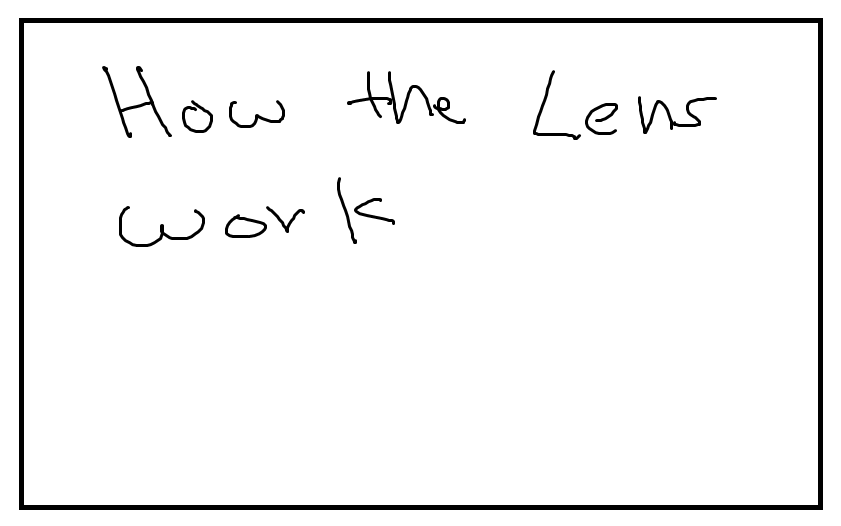
\includegraphics[width=\columnwidth]{lens_schematic.png}
	 \caption[Lens Widget Schematics]{Cross section schematics of the Lens Widget}
	 \label{figure:lensSchematic}
	\end{figure}
	% ==================


    % ===== Figure =====
	\begin{figure}
	 \centering  
	 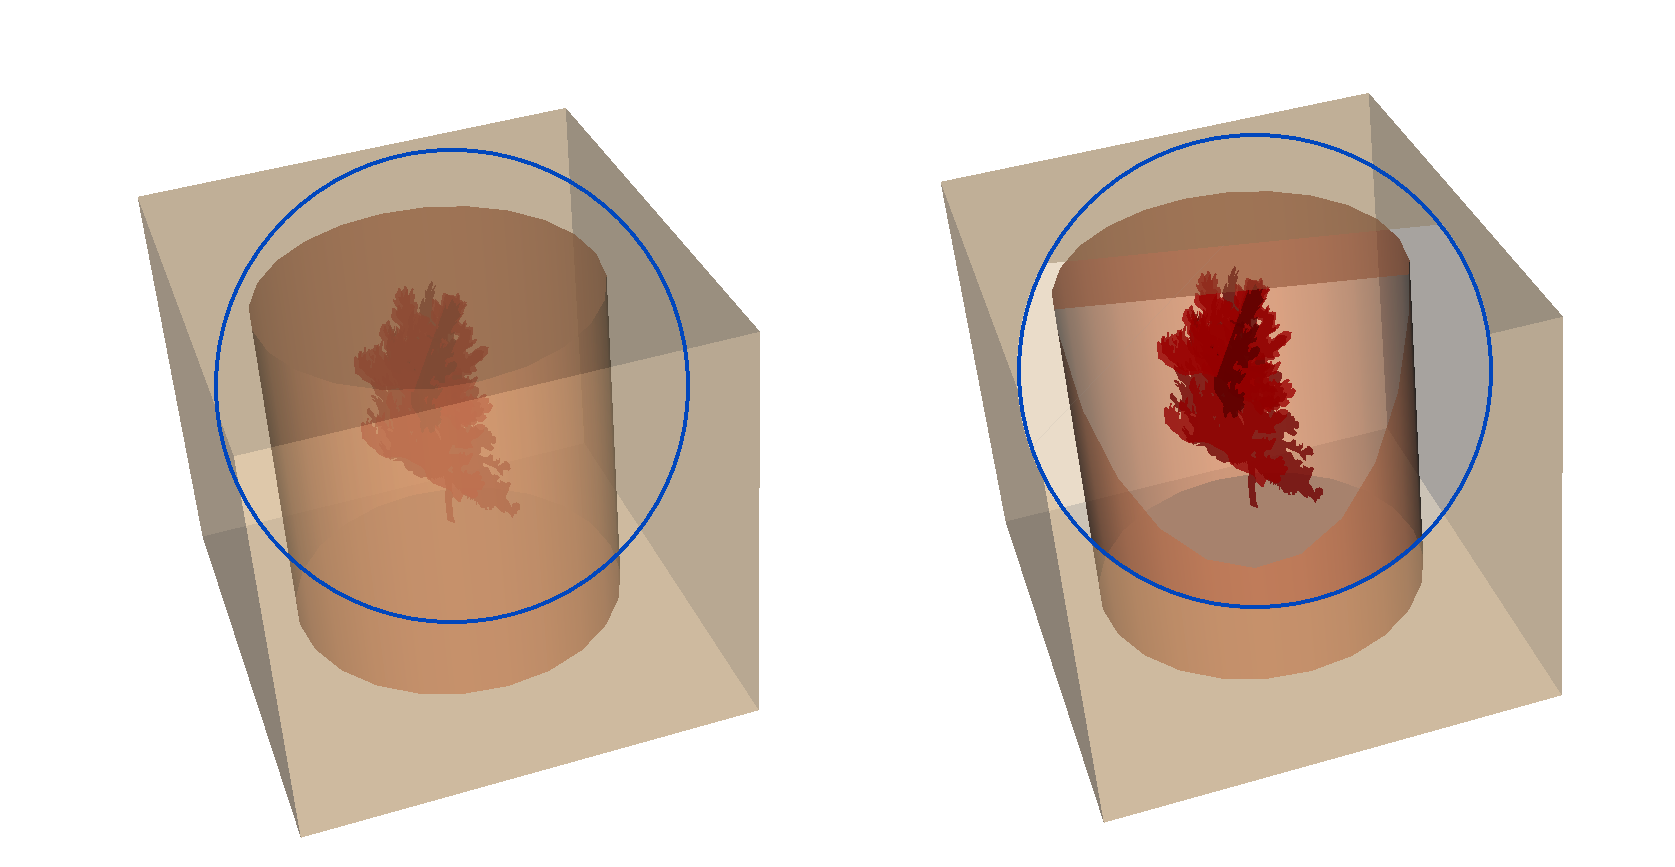
\includegraphics[width=\columnwidth]{lens_example.png}
	 \caption[Lens Widget in Action]{On the left, using the Lens Widget to expose
	 underlying semantics.
	 On the right, adjusting the depth field to cull away occluding geometries.}
	 \label{figure:lensExample}
	\end{figure}
	% ==================

The lens widget utilizes its own rendering pipeline, object geometries are
sent into the pipeline as normal, the rasterized result is then stored in an
intermediate buffer and later combined in fragment shaders with the default
rasterization scene. This is an independent process, and thus allows us to
render the lens' scene in different rendering styles and semantics. To visualize
the lens widget itself, we draw a semi-transparent border around its
circumference so viewers are aware of its existence. When interacting with the
lens widget, the widget is active and we render the border in blue, otherwise we
use the default grey colour. The semantics of the lens is not impacted by
whether the lens is active or inactive.

Three different types of interactions can be performs on the lens widget. The
position of the lens can be moved around the display, which impacts the
currently selected filters and the heatmap charts. The lens can be resized,
which increases or decreases its querying area. Lastly, a depth field can be
adjusted, this field acts as a cutting plane that removes entity objects that
comes before the plane. The depth field function provides a method for people to
reduce occlusion, as all entities that are the cut by the plane drawn in
an outline style that allows viewers to see into the object. Objects that are
cut off are excluded from any scoring calculations, they also have their
heatmaps hidden to reduce visual clutter. These three interactions can be
combined together to create a rich, flexible query mechanism.

Multiple lens widget are allowed for vacillating simultaneous explorations of
different parts of the visualization. For example, if the subject matter is of
an elongated shape, it is possible to use two lens to explore the entities
positioned at either end. However, we have not defined any semantics for
multiple lens to co-exist in the same spatial location, that is, the lens widget
has no defined behaviour when it is overlapped with another lens.

%To build a rich, flexible query mechanism, the position of the lens and the
%radius can be altered, thus creating different querying volume in different 
%spatial locations. In addition, each lens widget use a depth parameter that acts 
%as a cutting plane, all objects that comes before the cutting plane are excluded 
%from the tagging process and are rendered as inactive objects. The depth parameter 
%allows people to investigate occluded objects without resorting to changing their 
%viewing perspectives.

%Multiple lens widget are allowed to facilitate simultaneous exploration of
%different areas, for example if we are looking at a tower structure, we can one
%lens examining the base of the structure, while another lens examining the top of
%the tower. However we have not defined any semantics for the lens to overlap, thus 
%each lens should be used individually.


\subsection{Heatmap Widget}
The heatmap is an interactive widget that shows entity specific information over
the selected time frame. Each heatmap is designed to communicate how the volume
of complaints changed over time for individual entity components by fitting a
time series data onto a two dimensional grid. In particular, the heatmaps allows
year-to-year and month-to-month comparisons.

%The information chart extruded from the lens widget is designed as a
% heatmap-like chart, it shows the volume of complaints registered against individual objects 
%across time. Like our design for the time slider histograms, our intention is to 
%allow people to compare specific periods of time across different years for a 
%specific objects, albeit in finer detail. 

Prior to our heatmap implementation, we have also considered using a simple 
scatter-plot approach, with time on the X-axis and the volume of complaints on
the Y-axis. While this solution is simpler to read and likely easier to detect
long term trend, its major drawback is that it is likely more difficult to
make seasonal comparisons. For example, imagine a case where we want to compare
summer to fall over a 4 year span, one must constantly make the context switch
to decipher which parts of the graph represents summer, and which parts
represent winter. Also, in extreme cases scrolling need to be utilized for very
long time frames.

We arrange the time segments chronologically onto a grid like a calendar,
the month are arranged left-to-right in ascending order, and the years arranged 
top-to-bottom in ascending order. Each cell then represents the entity score for
the particular month. We use the same 6-bin colour encoding for the heatmap
widget to keep a consistent colouring scheme throughout the system. The widget
label, from left-to-right, shows the entity name, the number of complaints
referring to the entity with respect to the current query, and the number
of complaints in total if nothing is selected. Due to the use of synsets, each
entity has at least one corresponding string representations, we use the first
lemma that appears in our vocabulary, which may differ from actual text.

When examining the heatmap, trends and outliers can be detected visually. The
grid view aligns both month and year time dimensions, allowing viewers to
compare year and month with relative ease. Hovering over individual cells will cause a
tooltip to appear, showing the precise numerical score for the month, the tooltip itself is 
rendered with a semi-transparent style to avoid occlusion. Hovering also creates 
a visual cue of a highlighted border around the selected cell, the highlighting
effect is carried across all visible heatmaps as a brush+link effect.

With respect to the actual placement of the heatmaps, we have considered two
types of labeling layout for our lens widget: A flush-left/flush-right layout
that places the heatmaps on either left or right side of the lens, and a radial
layout where each heatmap is placed around the lens� circumference. The radial
layout is anchored at the centre of the lens, imaginary line segments extends
from the centre through the projected centroids, and a real line segments
extends the imaginary line to the circumference. The result was eye-pleasing,
but due to the nature of the lens being an exploratory tool which is moved
around the screen frequently, the layout is unstable and not suited for this
particular usage case. For the flush-based layout, we first sort the object
centroids by their Y-coordinates in screen space, then we place the heatmaps on
left/right side based on the heuristics below. Since there is no reliance on the
centre of the lens for placement, movement of the lens widget will not cause
drastic changes to the heatmap placement and thus produce a more stable looking
layout. Lastly we horizontally align the charts so it is easier for people to
compare values across different heatmaps.

In order to avoid occluding the \threed visualization, or to run off screen
space, we employ the following heuristics for heatmap placement.
\begin{itemize}[noitemsep]
  \item Heatmap placement should always be outside of the axis-aligned bounding
  box (AABB) in projected screen space of the \threed visualization, unless the
  AABB itself runs off the screen.
  \item If the heatmaps are off the screen space, perform contraction to move it
  back into screen space.
\end{itemize}

Because of limited screen space, we have made the decision to cap the number
of heatmaps that can be displayed at any given time. Rather than showing
heatmaps for all the entities under the lens widget, which would
inevitably create visual clutter, we employed a scrolling mechanism that 
allows people to scroll through the entities under the lens. We have a parameter
N which controls the maximum number of visible heatmaps. We have no
recommendations to what N should be, as it is tied to the amount of entities in
total, as well as the spatial placement of these entities. We found N=8 works
well with our vehicle complaint corpus.


\subsection{Document Widget}
The document widget is the final stage of our drill-down process by providing links 
to the raw text (Requirement R4). Each document is divided into two sections,
the header section shows each document�s fixed attributes and the content
section shows the raw text descriptions. We denote the selected entity words and
co-occurring entity words using blue and grey highlights respectively to create
contract against the remainder of the text. Scrolling is enabled with textual
content overflows the display panel, we use per-pixel based scrolling to ensure
fluid transition from document to document without any sudden disruptions.

We restrict the application to have a single document widget only. The widget is
toggle-based and is by default hidden from view. Once activated, an animation
will expand its dimension from a single pixel to its full size at the
activation coordinate, a reverse animation is used to deactivate the panel. Once
visible, a person can reposition the panel to move it to the desired location.


%%%%%%%%%%%%%%%%%%%%%%%%%%%%%%%%%%%%%%%%%%%%%%%%%%%%%%%%%%%%%%%%%%%%%%%%%%%%%%%%
\section{Interaction}
In this section we describe in greater detail how a person interacts with the
visualization by changing the underlying filters and using the widget to create
visually based queries. We also describe here our design for touch based
gestures, and visual feedback system for help people in their orientation of the
application.

%Interaction with the \threed model and interactive widgets dynamically update
%the visualization to reflect any changes. The change of visualization state is carried 
%through an animated transition that interpolates the colours and histogram values. 
%In this section we describe the high-level interactions and models that 
%support common tasks.

% This needs some work, it sounds kind of weird at places
\subsection{Entity Selection}
Entity objects can be acquired in two ways: One can directly select the entity
by performing the tap gesture on the \threed representation, or tapping the
heatmap through the lens widget. In the case where objects occlude each other
in \threed space, direct selection will return the object that is closest to
viewing point. In order to select occluded objects, the scene can be
rotated to reveal hidden entities. Alternatively, we can use the lens� depth
functionality to cut away occluding geometries, or directly clicking on the
heatmap representations which are always available.

Selection is toggle based. When an entity is selected, we apply a blue borderb
to the associated heatmap and the line segments that links the heatmap back to
the visualization. To visually accentuate the selection in \threed
space, we employ a halo like effect around the hull of the mesh objects. Both
selection and deselection of any entity triggers an event to recalculate the
entity scores, an animated sequence then starts to interpolate the colour of
each \threed object to reflect the scoring change.

The re-evaluation of the entity scores are based on current selection,
specifically they are recalculated based on their co-occurrence relation with
the current selection. Thus, highly co-occurring entities will score higher and
be more visible than lowly co-occurring entities.

Selection of an entity with zero score is considered invalid, instead, the
system will propagate the selection event through the zero scored entities.



%Selection is toggle based, thus clicking on a selected object or heatmap will 
%de-select that item. Clicking on an empty space will trigger a reset and de-select 
%all items. Selected items are accentuated visually with a glowing blue halo
%around the objects, this also applies to corresponding heatmaps which will have
%their border highlighted in blue. Any entities with 0 scores are considered
%inactive and are only drawn on the screen to give context, as such they are not
%selectable, any clicking on inactive object will cause the select action to go
%through the object to select the next nearest non-zero entity.


% This should be moved to the data section, probably. It talks about scores and
% how they are recalculated in co-occurring situations

%Selected objects are added to the selection buffer, which also act as a query
% filter.
%When selection buffer is not empty, object scores are calculated in relation to 
%the objects in the buffer, thus forming co-occurrence relations. For example, if 
%we selected the �engine� and �door� objects in the visualization, the rest of the 
%objects are recalculated to see if they co-occurs with both �engine� and �door�. 
%By this convention, the selected objects will always have the maximal score after 
%normalization, and will be coloured with the deepest shade on our colouring scale.

\begin{figure}
 \centering  
 \includegraphics[width=\columnwidth]{interaction_select.png}
 \caption[Interactive Selection]{The visualization changes based on the
 currently selected entities.}
 \label{figure:selection}
\end{figure}

 
\subsection{Spatial Interaction}
Traditional systems, particularly databases use explicit queries as a mean to
communicate with the underlying data. While this works well for task analysis,
it has an implicit assumption that the person knows something about how the
system works, and how the data is structured. Thus it can be a limiting factor
that prevents a wider audience from using applications without prior training.

Here we take a different approach, the lens widget allows people to demand and
filter detailed information by means of a visual query. Unlike explicit queries,
visual query is done more passively by moving the lens widget about the screen
to inspect different spatial areas that appear interesting to the viewer. This
is the key difference, as the focus selection is done visually, rather than
through explicit selection, this means the viewers do not need to know what the
entities are called to select them, reducing the need to have prior knowledge
about the data. This type of interaction is more playful and open-ended, people
are free to explore the visualization on their on terms which may lead to
unknown or unexpected discoveries.

In addition of the freedom to explore the visualization, the spatial
interaction has two other advantages: proximal relationship and reduced effort
in query construction. First, with most complex objects, incidents relating to
an entity is rarely in isolation, neighbouring objects are often impacted as
well. The lens widget allows selection of a volume range, which easily
facilitate bringing back entities close to the one we want to focus on. Second,
the visual query allows us to form queries that can be difficult to construct in
conventional systems. Imaging a case where we want to know how many vehicle
complaints are related to the ``front'' of the vehicle, traditional query would
require knowledge of the parts that belong to the front of the car, then follow
by an aggregation step of constructing a query that includes all these parts.
Our visual query simplifies this step by taking advantage of the familiar form
factor, a lens widget can be over the ``front'' of the vehicle visualization,
automatically pulling out all the relevant entities.


\subsection{Surface Based Interaction}
We use the idea of zone to segment our display space and to process touch
point events. Each zone consist of one or more polygonal spaces with predefined
semantics for handling touch based gestures. In the event that the zones overlap
each other and an event comes in, we only process the zone with the highest
priority. The priority of each zone is fixed and is predetermined. 

When a touch point is registered by the sensor hardware, we tie the touch point
to a single zone, the coupling will remain so until the touch point is removed.
The reason for this approach is to create a continuous interaction model, we
want to avoid sudden change of semantics which defies user expectations. This
approach also allows a subset of our dragging gestures(lens handle, slider
makers and scrolling) to continue to execute even if the actual touch point is
move off the predefined area, allowing higher tolerance for human error and
error recovery.

In the list below, we summarize the different zones we have in our application
\begin{itemize}[noitemsep]
  \item Visualization Zone: The main visualization, handles selection
  and deselection semantics of \threed objects, as well as heatmap selection.
  \item Time Zone: Covers the year and month time sliders 
  \item Filter Zone: Covers the organizational hierarchy filters
  \item Lens Zone: Handles semantics for change the physical attributes of a
  lens widget
  \item Document Zone: Covers the document widget
  \item Empty Zone: An empty zone is specially designated zone that is none of
  the above. Empty zone handles gestures related to camera and miscellaneous
  functions.
\end{itemize}


While we tried to adhere to commonly accepted gestures for navigational and
selection based tasks, our gesture design is also influenced heavily by our
hardware and our perceived usage scenario: an infrared sensor overlay placed
atop a large, nearly vertical display screen. Our hardware setup has several
design implications. The infrared sensor is imprecise because it senses
movements instead of real touches, as such it is possible to introduce
false positives due to how the hand posture and orientation. We can use software
heuristics to mitigate the consequences of these unintended noises, however,
there are ambiguous cases where we cannot guarantee the correct outcome. For example,
imagine a single handed gesture with the thumb and index finger, we have
noticed through experimental trials that the knuckles on the other fingers are
often picked up as extra touch points as well due to their proximity to the
sensor. In this case, it is difficult to judge which points are intentional and
which ones are not; these points are roughly equal distance apart, and without
additional information such as a camera image or depth which may be used to
conjecture hand orientation, we cannot guarantee correctness as we only have
Cartesian coordinates as our data source. Due to said reason, we decided
to abandon any complex, explicitly-singled-handed, multi-fingered gestures in
favour of a simpler, less error prone approach.

Our final gesture set is a cumulation of several iterations of redesign, new
heuristics and refinement of existing gestures. We pilot-test each iteration by
asking people to perform sample tasks and observer their reactions, in a few
cases we gave no instructions on how to use the system in order to observe their
natural instinct.

In our current iteration, we designed two types of touch gesture semantics for
our system: a tap semantic and a hold semantic. The tap semantic results from a
single touch where there is no delay between the initial touch gesture and
subsequent actions, conversely the hold semantic requires the user to hold the
initial touch point briefly before transitioning into subsequent movements. We
map the tap semantic to actions to selection, scrolling and orientation logic.
For the gestures that use the hold semantics, we reserve these gestures for the
toggling our custom made user interface widgets. 
We summarize our gesture set
below, group by by functional areas:
\begin{itemize} [noitemsep]
  \item Perspective Manipulation: Perspective manipulation consist of rotation
  of \threed model and camera zoom. Rotation is achieved with a
  single point horizontal or vertical drag gesture, which corresponds to
  rotation of the XY and XY planes. Zooming events are triggered by bringing
  together two touch points closer together or further apart. All perspective
  manipulations are restricted to the empty zone.

  \item Entity Selection: Entity selection is triggered with a single tap event.
  A hold gesture on an entity will invoke the tooltip widget, if applicable.
  
  \item Time Sliders: Single-tap gesture is used to send select events to
  individual time sliders. Dragging gesture is used to move the markers left and
  right for selecting multiple periods.
  
  \item Hierarchical Filters: A single tap gesture is used to open, close and to
  make selections. Scrolling is achieved by dragging the item list vertically.
  Note the gestures are associated with unique events, thus we do not allow
  transition from one semantic to another, even though the gesture point is on
  the same zone. For example, one cannot transition directly from dragging the
  item list to select, a separate gesture need to be executed to perform the
  selection.
  
  \item Lens Manipulation: A lens widget is created by specifying its diameter
  with two hold points, for example using index fingers on left and right hand
  to create the diameter. We impose a minimum and maximum diameter length to
  keep the physical size of the lens within reason, with our display hardware,
  we use the range between 100 to 500 pixels. Dragging gesture performed on the inner part
  of the lens shift the lens location, while dragging gesture performed on the
  border resize the lens with respect to the point's distance away from the
  lens centre. A resize that results in a diameter that falls below the minimum
  threshold removes the lens widget from the application. The handle on the
  widget adjusts the depth parameter, dragging the handle counter-clockwise
  increases the cutting depth, while the reverse decreases the cutting depth, we
  modelled this behaviour after the zooming mechanism on the barrels of camera
  lenses.
  
  \item Text Browsing: The document panel becomes active upon a hold gesture
  event, with no other hold events in its vicinity. The hide the panel from
  view, executing a hold gesture anywhere on the document widget will trigger
  the close event. The widget is further subdivided vertically into two separate
  zones at 80 percent and 20 percent of the widget's width. The larger of the
  two listens to move events, while the smaller one, positioned on the right
  side handles scrolling of text. Both of these zones receive tap based
  events.
  
\end{itemize}



\subsection{Visual Feedback}
When using the keyboard, mouse and other hardware peripherals, actions are
rewarded with some type of haptic feedback, for example we know when a key on a 
keyboard is pressed of depressed. This behaviour allows people to be more keenly 
aware of the system's current state. This is not true with touch interfaces,
with touch sensing technology, it is possible for touch points to become lost during a gesture, 
this is due to the users accidentally lifting their fingers. When this happens people 
can get confused because they may be not be aware that their touch points are lost 
since their fingers are still contacting the table, there are no feedback system 
to alert the actual touch point had disappeared. To accommodate the lack of
physical response, we implemented out own visual feedback system. We created
four different types of visual cues, which we summarize below and can be seen in
Figure \ref{figure:feedback}. 

\begin{itemize}[noitemsep]
  \item Touch Point: Whenever a touch point is registered, we render a gradient
  circle at the XY screen coordinate as detected by the infrared sensor. The
  radius of the circle is slightly larger than the average finger tip such that
  is is always visible, this is about 15 pixels on our display. The position of
  the gradient circle is updated in-sync with the sensor updates, and is removed
  when the touch point is rescinded. This visual cue gives viewers immediate
  feedback of the active touch points, which can be used to perform higher level
  actions.
  \item Hold Point: A hold point has the same basic visual cue as a touch point.
  A hold point starts off as a touch point, a ticking timer running in the
  background determines when the touch point transitions into a hold point. We
  visualize this timing sequence as a arc outside of the circle, the arc grows
  with an increasing central angle and opacity that are mapped to the amount of
  time required to become a hold point. A hold gesture is activated once the arc has travelled
  the entire circumference and lock down. An interruption during the transition
  phase will remove the animation, the gesture will return back to a normal
  touch point.
  \item Trails: Our system keeps track of previous updates for a single,
  uninterrupted point. We visualize up to the last 10 most recent updates as
  breadcrumb trails to serve as a reminder of what type of high level gesture is
  being performed. The XY coordinates of previous update points are drawn in
  smaller circles, similar to that of touch points.
  \item Removals: These visual cues are used to denote any removals sensed by
  the hardware device, these includes the active points sensed by our software
  and also any other ones that were rejected by our evaluating heuristics. This
  cue gives the viewers some sense of the hardware capabilities and
  deficiencies. We think this is useful as a learning device, viewers are able
  to see where they may inadvertently cause unwanted touch points and use this
  experience to adjust how they operate their gestures next time they interact
  with the system. We visualize this as circular outlines that decrease in
  opacity and radius with time, they are removed from the system when the radius
  reaches zero.
\end{itemize}
 
 
\begin{figure}
 \centering  
 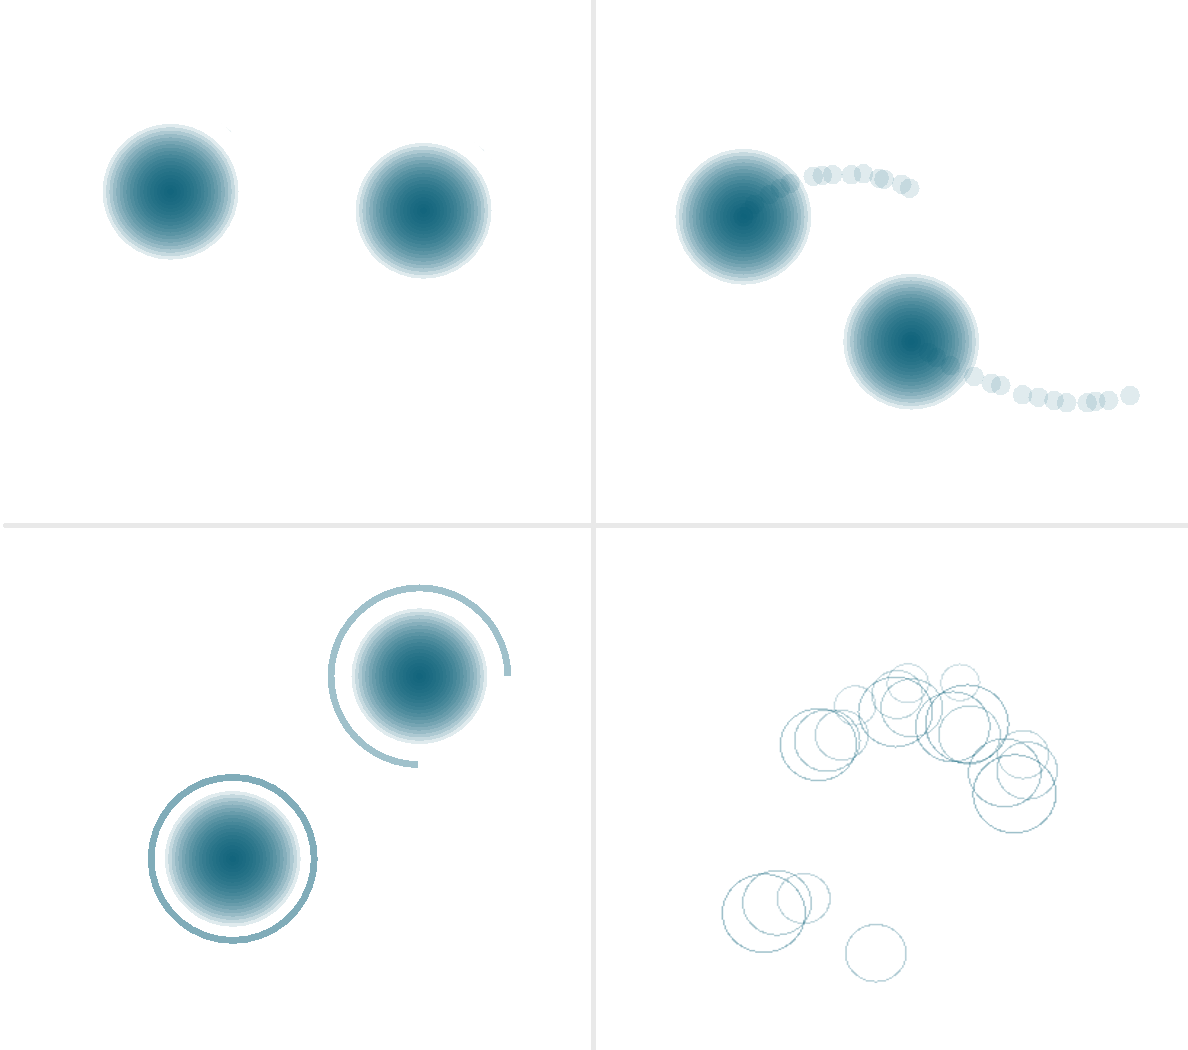
\includegraphics[width=\columnwidth]{feedback.png}
 \caption[Visual Feedback]{Different visual feedback to help viewers
 differentiate different system states}
 \label{figure:feedback}
\end{figure}



%%%%%%%%%%%%%%%%%%%%%%%%%%%%%%%%%%%%%%%%%%%%%%%%%%%%%%%%%%%%%%%%%%%%%%%%%%%%%%%%
\section{Viewing Modes}
A comprehensive analytic system requires a variety of ways to manipulate and
looking at data. In this section we describe our solutions for trend detection,
making comparisons and high level overview.

\subsection{Heatmap Perspective}
The heatmap�s data, in essence, is a time series data. There are multiple ways
we can view this time series to derive interesting patterns and trends. For this 
prototype we want to concentrate on comparability across different components
and time. For example, we want to ask: which vehicle component had more
complaints? which month had more complaints out of the year? 
To do this, we need to have multiple perspectives where data can be viewed from
different functional needs. We have provided the following perspectives in our
prototype:
\begin{itemize} [noitemsep]
  \item Month-Max: A monthly perspective where the importance score of each
  month is divided by the maximum monthly importance score over all components
  in the selected time.
  \item Component-Max: An object component perspective where the importance
  score of each month is divided by the maximum component score over the selected time.
  \item Global-Max: A global perspective where the month score is divided by the
  maximum score of all components over the selected time. 
\end{itemize}
Each of the perspectives above answers different questions and has its own
advantages and disadvantages. The month-max perspective allows us to compare 
component-to-component by month, but comparison against adjacent cells are 
meaningless because each cell uses a different base value. The component-max 
perspective is the opposite, it allows us to see trends with a single entity, 
but it does not allow comparison across components. Lastly, the global-max 
perspective is good at showing the outliers and supports both month-to-month 
and component-to-component comparisons, but it can be difficult to see any
trends  in the non-outlier data because they are pushed into the bottom bins on 
the colour scale. To put the different modes in better context, we list sample 
questions that can be answered with these different perspective views:
\begin{itemize} [noitemsep]
  \item Month-Max: In month X, which vehicle component had the most complaints?
  \item Component-Max: Are there more braking problems in the summer months or
  the winter month?
  \item Global-Max: What are the most unreliable vehicle components?
\end{itemize}
We had some considerations on whether to make the perspective a localized
setting or a global setting. A localized perspective could be attached to aa
lens widget, allowing more flexibility, but at the same time introduces more
complexity because the reader will have to deal with multiple modalities
simultaneously. A global setting makes it clear what perspective is being used,
but cause global changes even when the reader only wants to query a single
entity. In the end, we decided that localized perspective may cause too much
confusion for our users. We made the perspective mode a global setting, via a
drop-down list located at the bottom left of the user interface.


\begin{figure}
 \centering  
 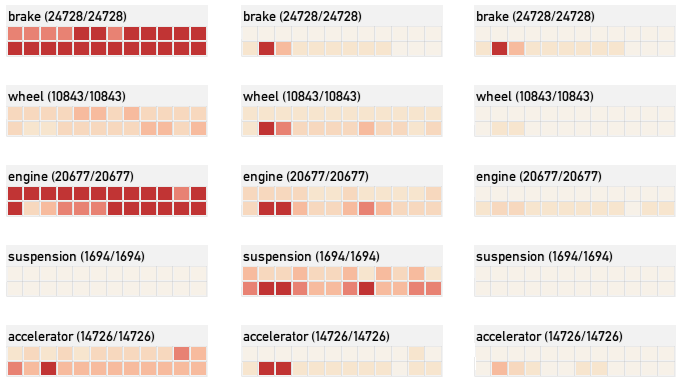
\includegraphics[width=\columnwidth]{heatmap.png}
 \caption[Heatmap Perspectives]{Showing the different heatmap perspectives. Left
 displays the monthly perspective, centre displays the component perspective, and right displays the
 global perspective}
 \label{figure:heatmap}
\end{figure}

\subsection{Comparison}
Comparison mode allows people to compare two different types of the same
physical product specified by two different query sets Q1 and Q2. Every entity
from a query set is matched against the same named entity in the other query
set, producing an entity level based comparison. For example, we can compare how
each car component fared against each other in a comparison of Honda Civic
versus Toyota Corolla, or comparing Ford Focus against the industry form.

Two separate measures are used for the comparison view. A contribution sum and a
percentage difference. The contribution sum is the aggregated entity score from
the two query sets, it reflects the overall importance of the entity by
emphasizing the frequently occurring entities in one or both query set. The
percentage difference describes the relative frequencies of an entity, whether
it occurs more frequently under Q1 or Q2 relative to the total contributions
from Q1 and Q2 respectively. The percentage score is calculated as entity score
divided by the total contribution. Then the percentage difference follows as
percentage score Q1 minus percentage score Q2, with the sign and magnitude
indicating  which query set has the stronger presence. We made the decision to
use percentage based comparisons because it enables as to compare query results
of different sizes.

We encode the sum score as the colour of the \threed component, based on the
default colour scale. For the difference, we render the measure as an outline
around the object. The sign of the difference is encoded as one of two diverging
colours, one for positive and one for negative values. The magnitude of the
difference is encoded as the transparency of the outline, larger magnitude have
more distinct, solid outlines compared to smaller values. Thus, a highly
problematic object from both side will have a strong presence overall but with a
faint outline, while a lopsided but infrequent problem will have strong outline
but barely visible interior colour.

 
\begin{figure}
 \centering  
 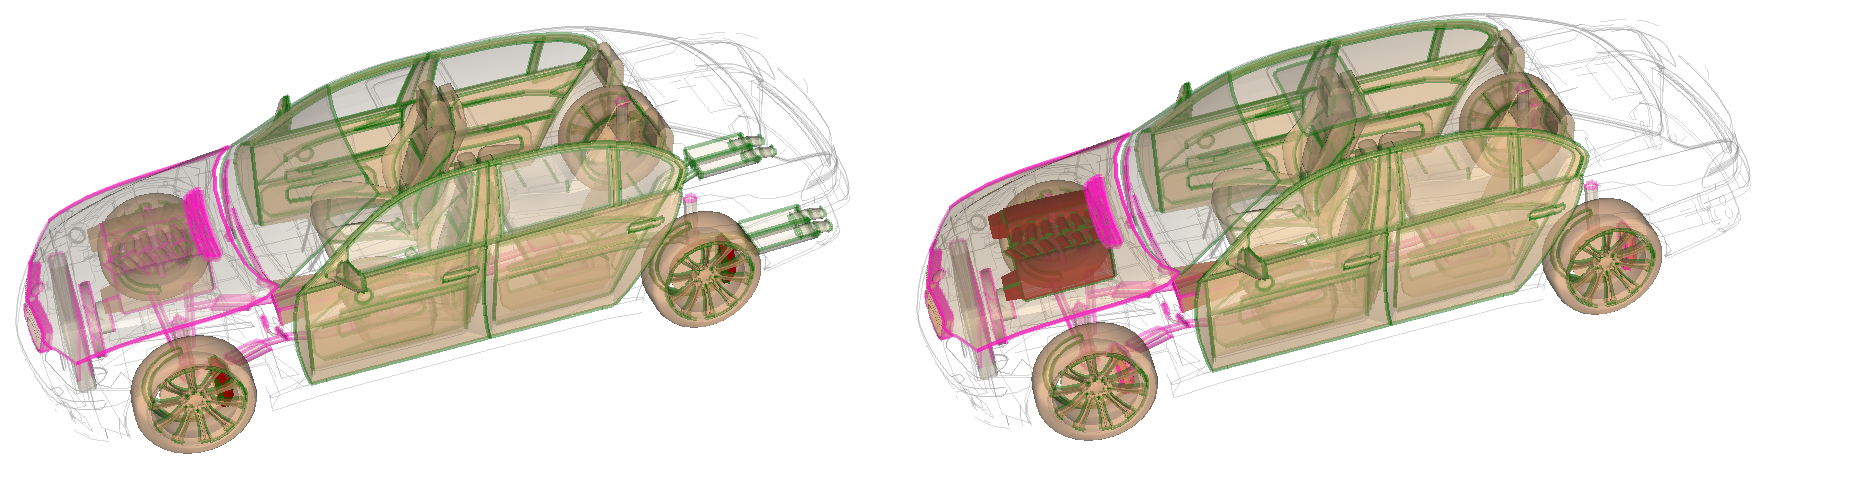
\includegraphics[width=\columnwidth]{comparison.png}
 \caption[Comparison View]{Comparison View}
 \label{figure:comparison}
\end{figure}

By default, comparison mode is turned off. It is activated when the viewer
switches the second hierarchy filter from the ``None'' position to a valid
selection. Subsequent query modifications are carried out in comparison mode
until the selection is turned to ``None'' again.

One limitation with this approach is our current usage of the total
contributions to calculate the percentage scores. Our total contribution is in
relations to the number of documents in the corpus, which may or may not be a
good indication of the overall contribution. 


%The of the limitation in the current prototype is that we do not have any
%normalization of comparative scores, thus it only makes sense comparing two 
%different types of products with similar volumes.

\subsection{Aggregation}
By default, the system treats each object individually rather than object
groups. For example ``seatbelt'', ``backrest'' and ``seat'' are all scored
separately, even though they are logically under the group ``seat''. This
setting allows people to isolate and identify unique problems accurately. There
are times, however, when this level of information is unnecessarily detailed and
a higher level overview is desirable.

Aggregation mode mimics the type of high level rating system found on consumers
review websites. When aggregation mode is enabled, individual objects, and their
scores are aggregated up to the first level entities. In our specific case, the 
first level are the major sub-systems in a vehicle. The visualization responds
by making all child objects referencing the aggregated score of their parent
subsystem. 

Aggregation mode is enabled/disabled by a toggle switch located at the bottom
left of the user interface. Aggregation mode works in conjunction with
comparison mode, allow people to make comparison of major systems.
 
\begin{figure}
 \centering  
 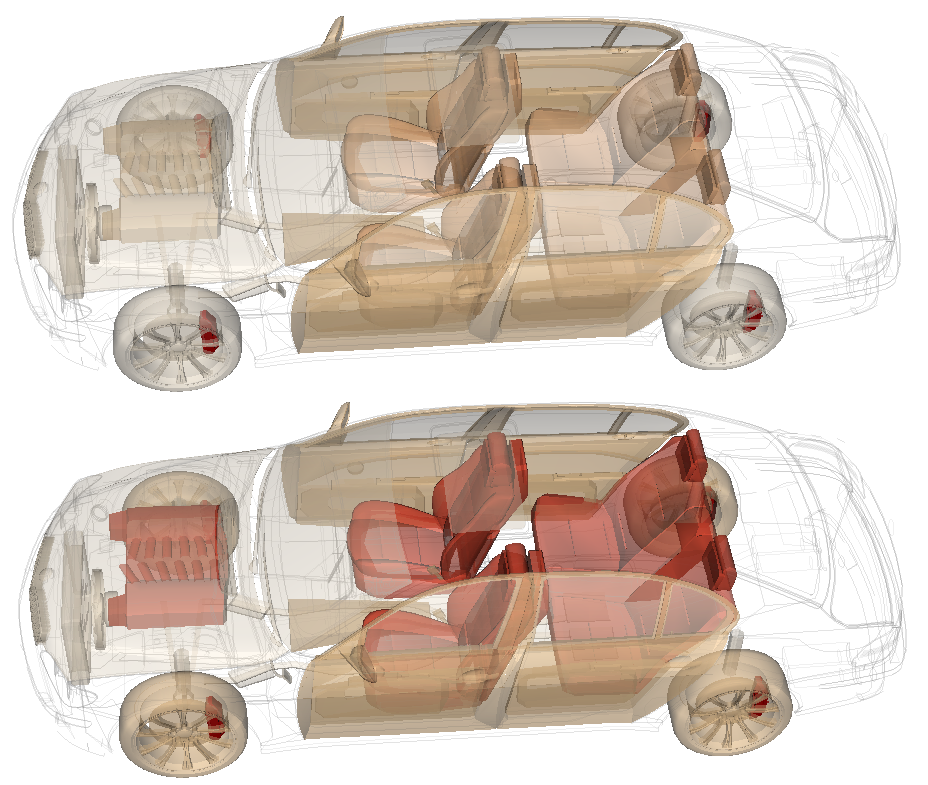
\includegraphics[width=\columnwidth]{aggregation.png}
 \caption[Aggregation View]{Top: Aggregation mode disabled. Bottom: Aggregation
 mode enabled, note that the seat and engine now appears more prominent in the visualization.}
 \label{figure:heatmap}
\end{figure}
